\section{Comparaciones}
Para analizar el comportamiento de las estrategias, generamos distintos patrones de
acceso a la base de datos (trazas). Corrimos las diferentes estrategias para cada traza,
haciendo variar el tamaño del Pool. Para cada una de estas corridas, calculamos el 
hitrate de cada estrategia. Luego representamos estos resultados en gráficos comparativos
que utilizamos para verificar nuestras hipotesis.

\subsection{Generación de Trazas}
TouchCount intenta resolver casos en los que tanto LRU como MRU, algoritmos predecesores, por lo que
generamos trazas imitando el comportamiento apropiado de dichos casos. Estas fueron generadas con
el mixer otorgado por la cátedra y con trazas previamente generadas. 

A continuación, se explica cada una de ellas

\begin{itemize}
\item{La primera traza combina distintos tipos de acceso pero con una relevancia mayor al FileScan. 
(referirse a Motivación de Touch Count pará más información)}
\item{La segunda traza, al igual que el anterior, combina otros tipos, pero esta vez su mayoría radica en IndexScan}
\item{La tercera traza realiza solo FileScan ya que es el problema principal a resolver dentro de LRU, y como se comporta delante la decisión de separdación del buffer en Hot Y Cold}
\end{itemize}

\subsection{Análisis}
Cada una de las trazas antes mencionadas fueron probadas ante distintos tamaños de buffer para comparar los HitRate obtenidos

\begin{figure}[ht] % htbp es para que lo tenga dentro del section
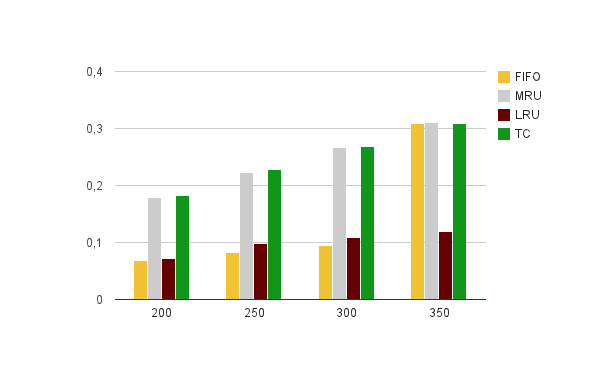
\includegraphics[scale=.80]{grafico1-1}
\caption{Mixed Trace con más File Scan}
Como veníamos prediciendo, Touch Count muestra una mejor performance frente al resto. 
Si bien las diferencias son pequeñas, se mantienen para los distintos tamaños.
\end{figure}

\begin{figure}[ht]
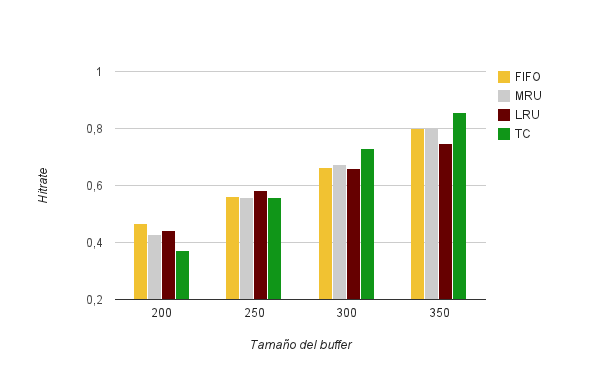
\includegraphics[scale=.80]{grafico1-2}
\caption{Random File Scan +File Scan}
En este caso para tamaños más chicos de Buffer, obtenemos mejores resultados con LRU y MRU. 
Como el paper indica, este Algoritmo fue pensado ante el nuevo avance computacional
de Buffers más grandes comparado cuando se empezaron a utilizar los algoritmos LRU y MRU, por lo 
que es lógico que, tal como vemos en el gráfico, TouchCount se comporte mejor ante tamaños de Buffer más grandes
\end{figure}

% \begin{figure}[ht]
% 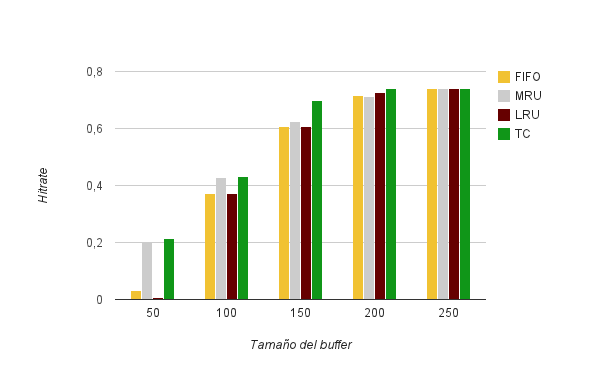
\includegraphics[scale=.80]{grafico2-1}
% \caption{Mixed Trace con más Index Scann}
% En este caso para
% \end{figure}

\begin{figure}[ht]
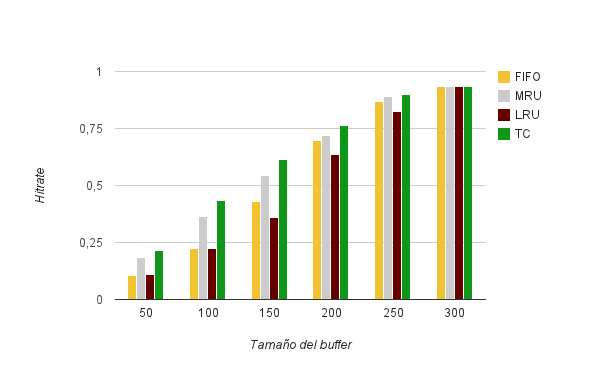
\includegraphics[scale=.80]{grafico2-2}
\caption{Mixed Trace +Index Scan}
Tanto como para el primer caso, el resultado predicho fue el ganador. Touch Count obtiene una mejor performance frente al resto.
\end{figure}

\clearpage

\begin{figure}[Ht]
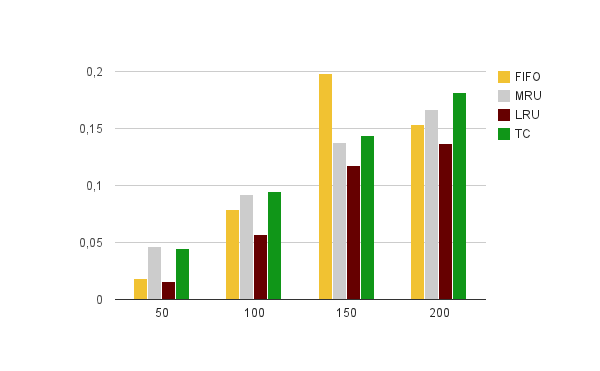
\includegraphics[scale=.80]{grafico3}
\caption{Mixed Trace solo File Scan}
Al ser todo FileScan, los algoritmos LRU y FIFO tienen problemas (referirse a Motivación de Touch Count pará más información), por lo que deberían dar casi 0 HitRate.
Y MRU y TouchCount deberían dar mejores valores. Esto se ve reflejado en el gráfico de arriba.
\end{figure}



\section{Conclusión}

Observando estos gráficos podemos observar que el Touch Count es el que tiene un comportamiento más regular en todos los casos. No obstante siguen existiendo combinaciones de trazas que tendrían un mayor hitrate si se utilizara MRU o LRU. Aunque el Touch Count nos demuestra que abarca una espectro mas amplio de casos podría inducirnos a que quizás siga existiendo espacio para mejorar la selección de
víctimas de un buffer pool. Una posibilidad sería el tratar de que el algoritmo identifique los casos en los que el touchcount no representa la mejor opción antes de aplicarlo.



